\section{Cryptographic Access Control}
\label{sec:background.cac}

In cloud-based applications, \gls{cac} can be used to ensure the confidentiality and integrity of data when the \gls{csp} is honest-but-curious. With \gls{cac}, all files are encrypted and freely distributed by the \gls{csp}, with the encryption ensuring that only authorized users --- which possess the secret decrypting keys --- can access the files. \Gls{cac} is an \gls{ac} mechanism that concretely solves the key distribution problem by implementing an \gls{ac} model using cryptography.
Garrison et al. proposed a scheme for applying \gls{cac} to \gls{rbac} \cite{cac}.
Their solution is described below. We assume that an authenticated and encrypted channel exists between each user and the administrator (e.g. using \gls{tls}). Each user \( \user \) and role \( \role \) has two asymmetric key pairs \( (\keyenc{}, \keydec{}) \) and \( (\keyver{}, \keysig{}) \) for en/decryption and for creating/verifying digital signatures, respectively. \( \keydec{} \) and \( \keysig{} \) are the private keys and \( \keyenc{} \) and \( \keyver{} \) are the public keys. 
The encryption/decryption key of the role is used to decrypt the key of the files.
Each file \( \file \) is encrypted with a symmetric key \( \key{}{\file.\fname} \), obtaining an encrypted file as \( \encsym{\key{}{\file.\fname}}{\file.\fcontent} \). To assign a user \( \user \) to a role \( \role \), the administrator of the policy encrypts the decryption and signing keys \( (\keydec{r}, \keysig{r}) \) of \( \role \) with the public key of \( \user \), i.e., \( \keyencu \), resulting in \( \encpub{\keyencu}{\keydec{\role}, \keysig{r}} \). To grant permission for a role \( \role \) to access a file \( \file \), the administrator of the policy encrypts the file's key \( \key{}{\file.\fname} \) with the public key of the role resulting in \( \encpub{\keyenc{\role}}{\key{}{\file.\fname}} \). 

To decrypt a file, the procedure is:
\begin{itemize}
	\item \( \user \) decrypts \( \decpub{\keydecu}{\encpub{\keyencu}{\keydec{\role}, \keysig{\role}}} \), obtaining \( (\keydec{\role}, \keysig{\role}) \);
	\item \( \user \) decrypts \( \decpub{\keydec{\role}}{\encpub{\keyenc{\role}}{\key{}{\file.\fname}}} \), obtaining \( \key{}{\file.\fname} \);
	\item \( \user \) decypts \( \decsym{\key{}{\file.\fname}}{\encsym{\key{}{\file.\fname}}{\file.\fcontent}} \), obtaining \( \file.\fcontent \).
\end{itemize}

The \gls{cac} scheme in \cite{cac} requires the storage of additional data, such as keys for en/decryption and for creating/verifying digital signatures, \gls{ac} policy status, and version numbers. These data are called metadata and are digitally signed. The metadata are organized into tuples, each of which is signed by the author. The provided tuples include: \texttt{RK}, which contains the \( \keydec{\role} \) and \( \keysig{\role} \) keys of a role signed with a user's key \( \keyencu \), \texttt{FK}, which contains the symmetric key \( \key{}{\file} \) of a file \( \file \) encrypted with a role's public key \( \keyenc{\role} \), and \texttt{F}, which represents the encrypted files. The \gls{csp} stores the encrypted data and metadata, while each user keeps their own key on their own secure device (e.g. laptop, smartphone, \gls{hsm}), assuming that the device is secure and that an attacker does not obtain the user's key.
%
% \begin{figure}[t]
	%     \centering
	%     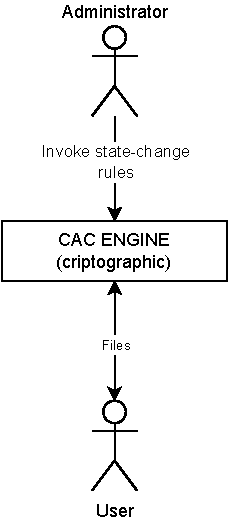
\includegraphics[width=0.15\textwidth]{assets/img/cac_scheme.pdf}
	%     \caption{\label{fig:cac_scheme}The hybrid scheme}
	% \end{figure}
%
Finally, \gls{cac} is conceptually composed of these entities \cite{berlato_formal_2021}:
\begin{itemize}
	\item \textbf{proxy}: this is software installed on the user's device that performs cryptographic computations (such as encryption, decryption, signing, verification, tuple generation, and verification) on behalf of the user. It also manages the keys;
	\item \textbf{metadata manager}: it stores the metadata (i.e., the tuples), the set of the metadata is the current \gls{ac} state;
	\item \textbf{data manager}: it stores the encrypted data;
	\item \textbf{reference monitor}: it receives the encrypted data and metadata from the proxy, verifies that the metadata is well-formed, signed and valid for the current \gls{ac} state. If all is well, it stores the metadata in the metadata manager and the encrypted data in the data manager.
\end{itemize}
